\section{ Detector Level Measurements }
\label{sec:DetectorLevel_Measurement}

\begin{figure}[!htb]
    \centering
    \begin{subfigure}{.49\textwidth}
        \centering
        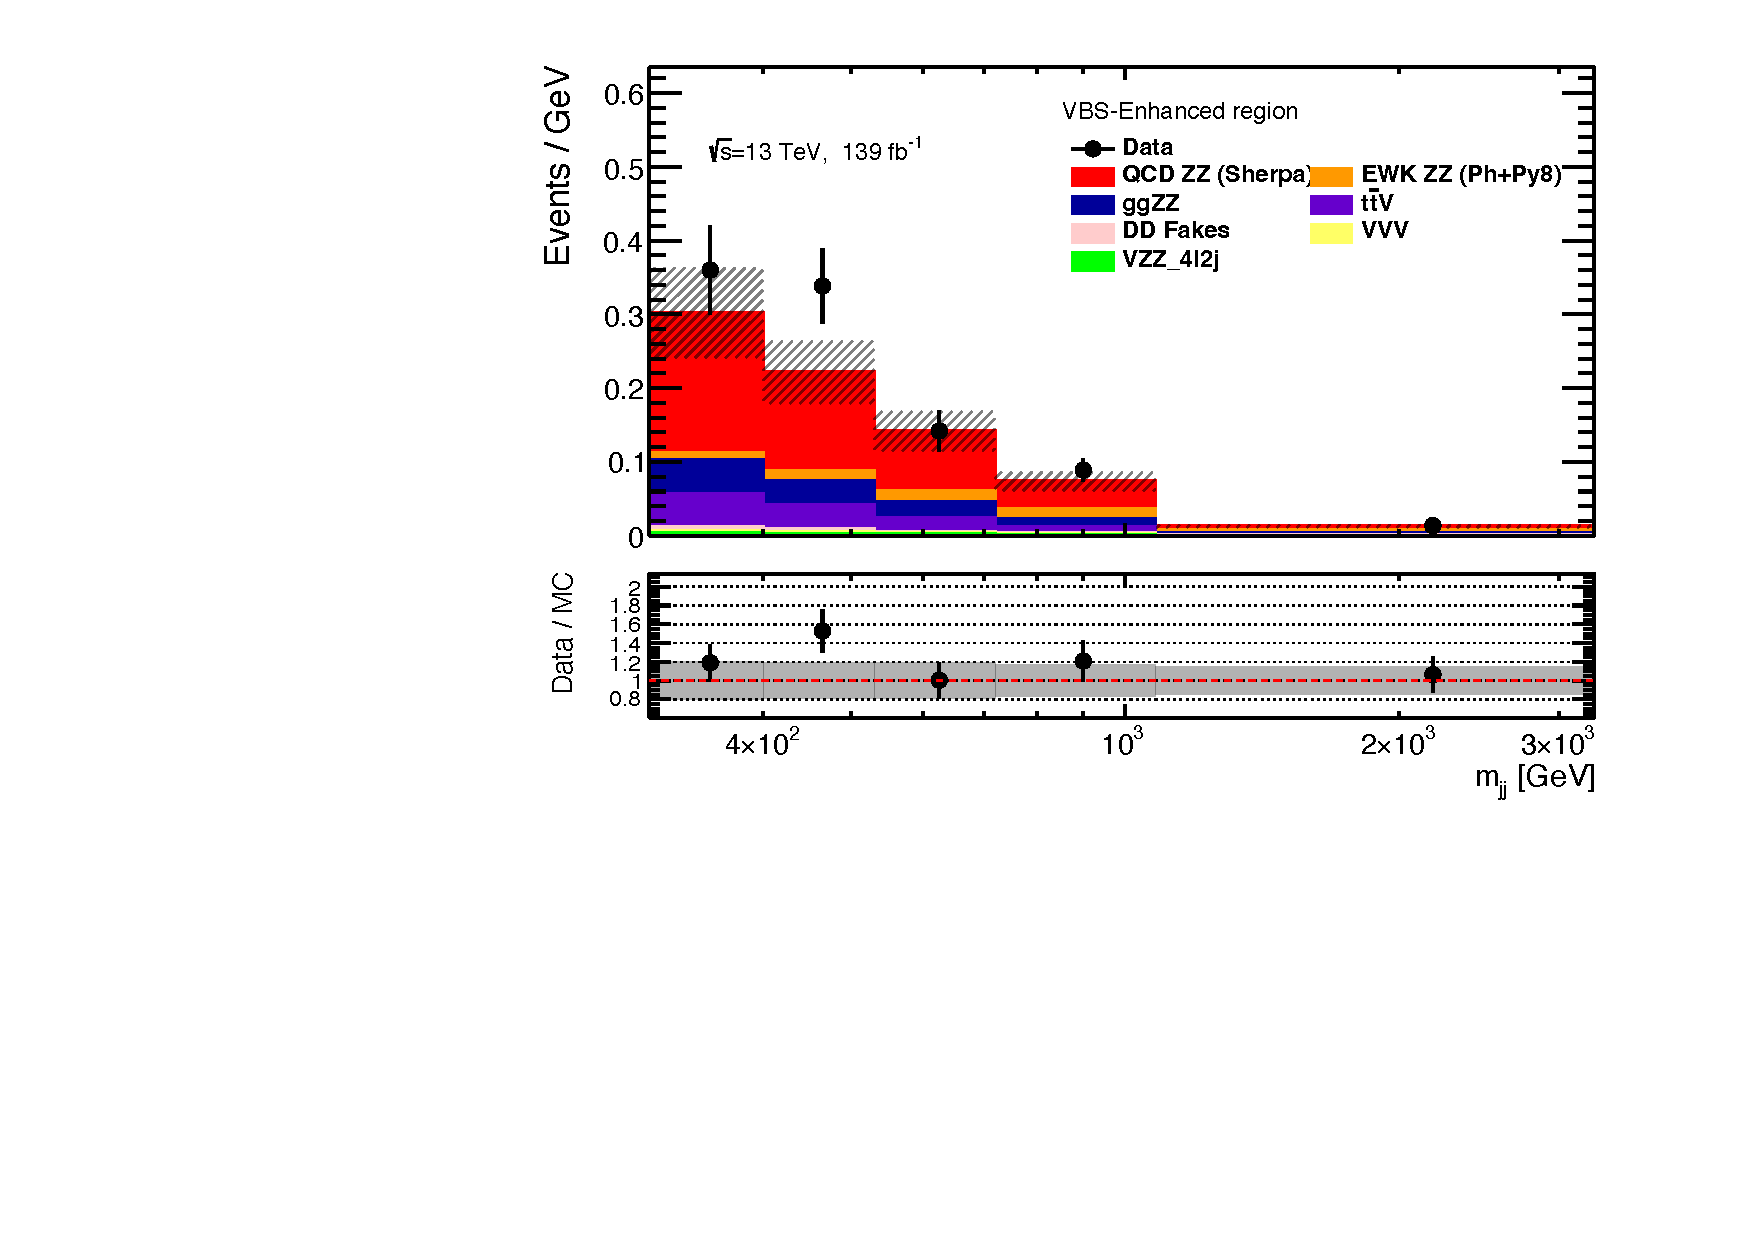
\includegraphics[width=.98\linewidth]{figures/Results/RecoDist_VBSEnhanced/reco_mjj_SR.pdf}
        \caption{ \footnotesize{$m_{jj}$}: $\chi^2/NDF = 0.43$ }
    \end{subfigure}
    \begin{subfigure}{.49\textwidth}
        \centering
        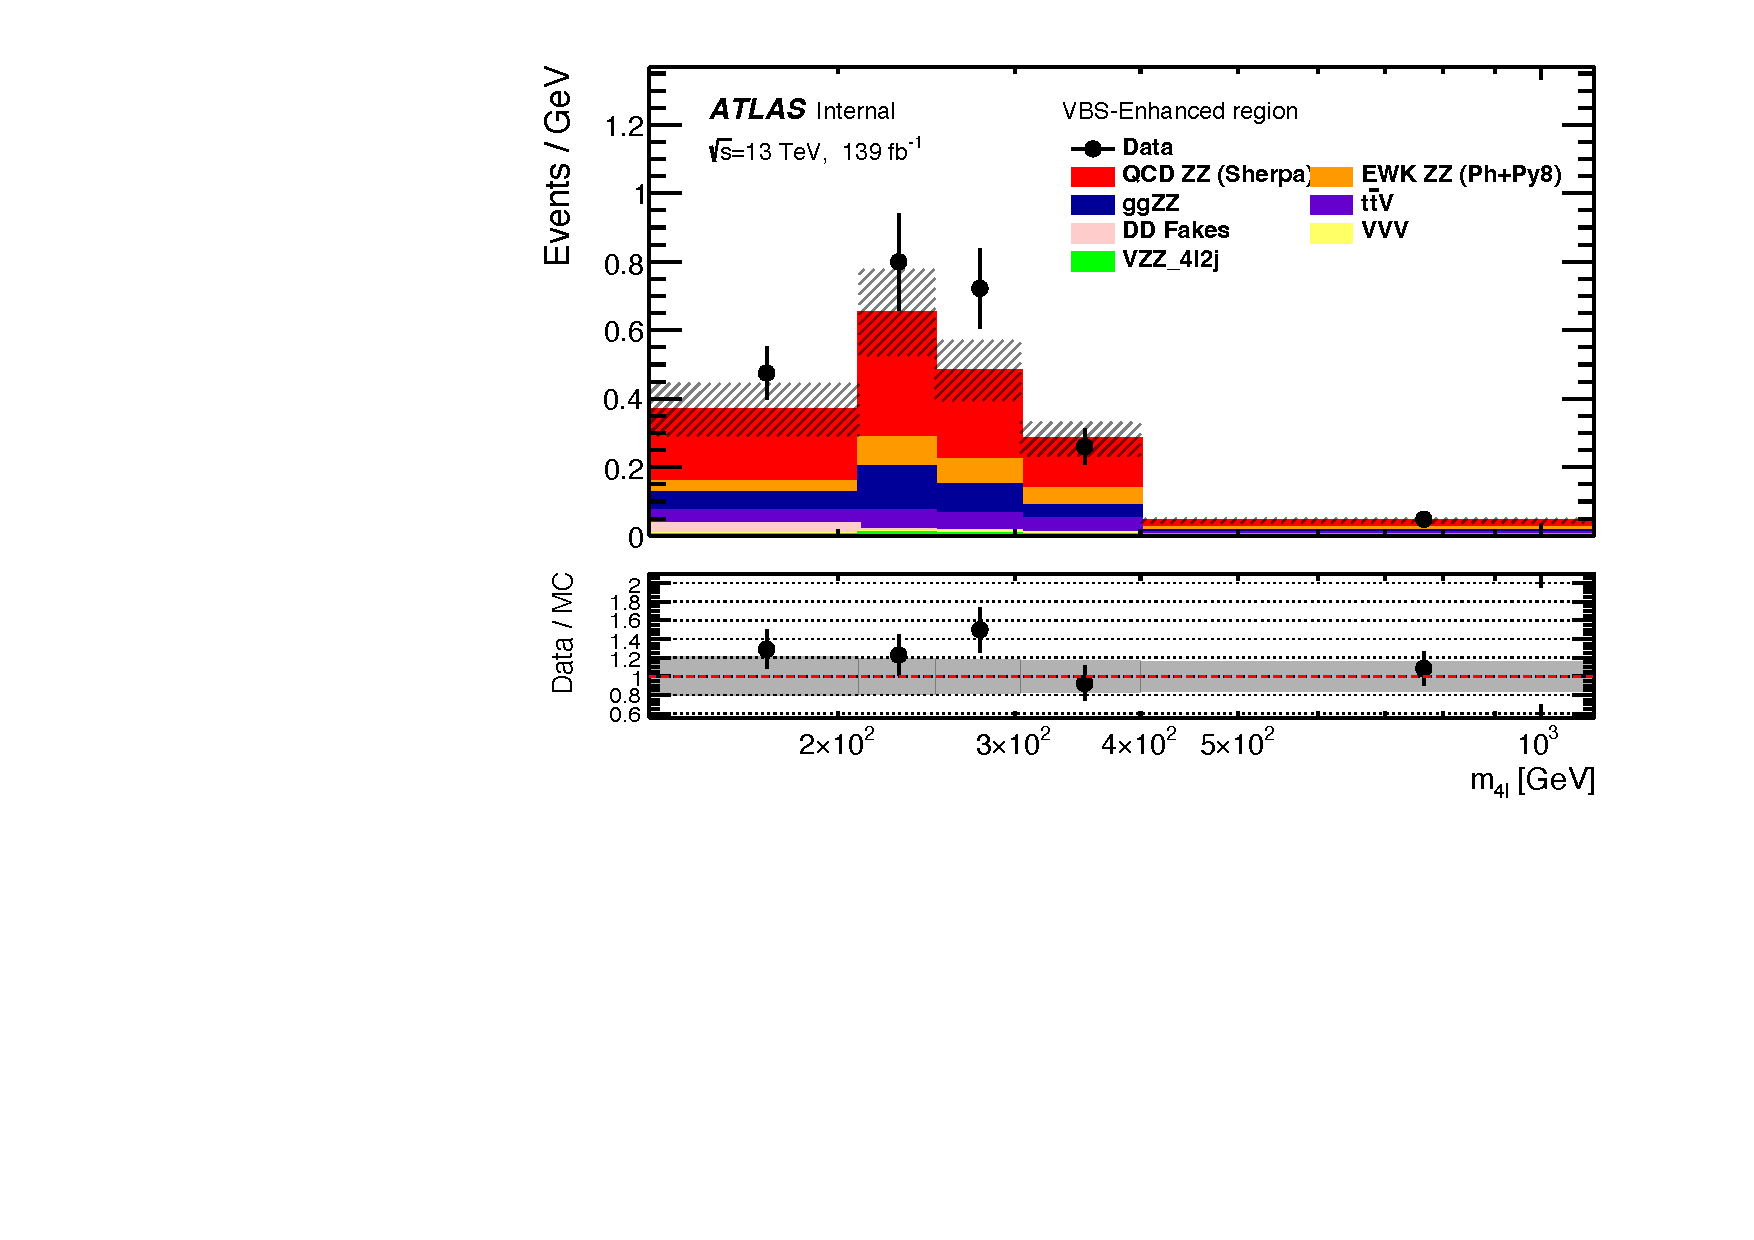
\includegraphics[width=.98\linewidth]{figures/Results/RecoDist_VBSEnhanced/reco_m4l_SR.pdf}
        \caption{ \footnotesize{$m_{4\ell}$ }: $\chi^2/NDF = 0.49$ }
    \end{subfigure}\\
    \begin{subfigure}{.49\textwidth}
        \centering
        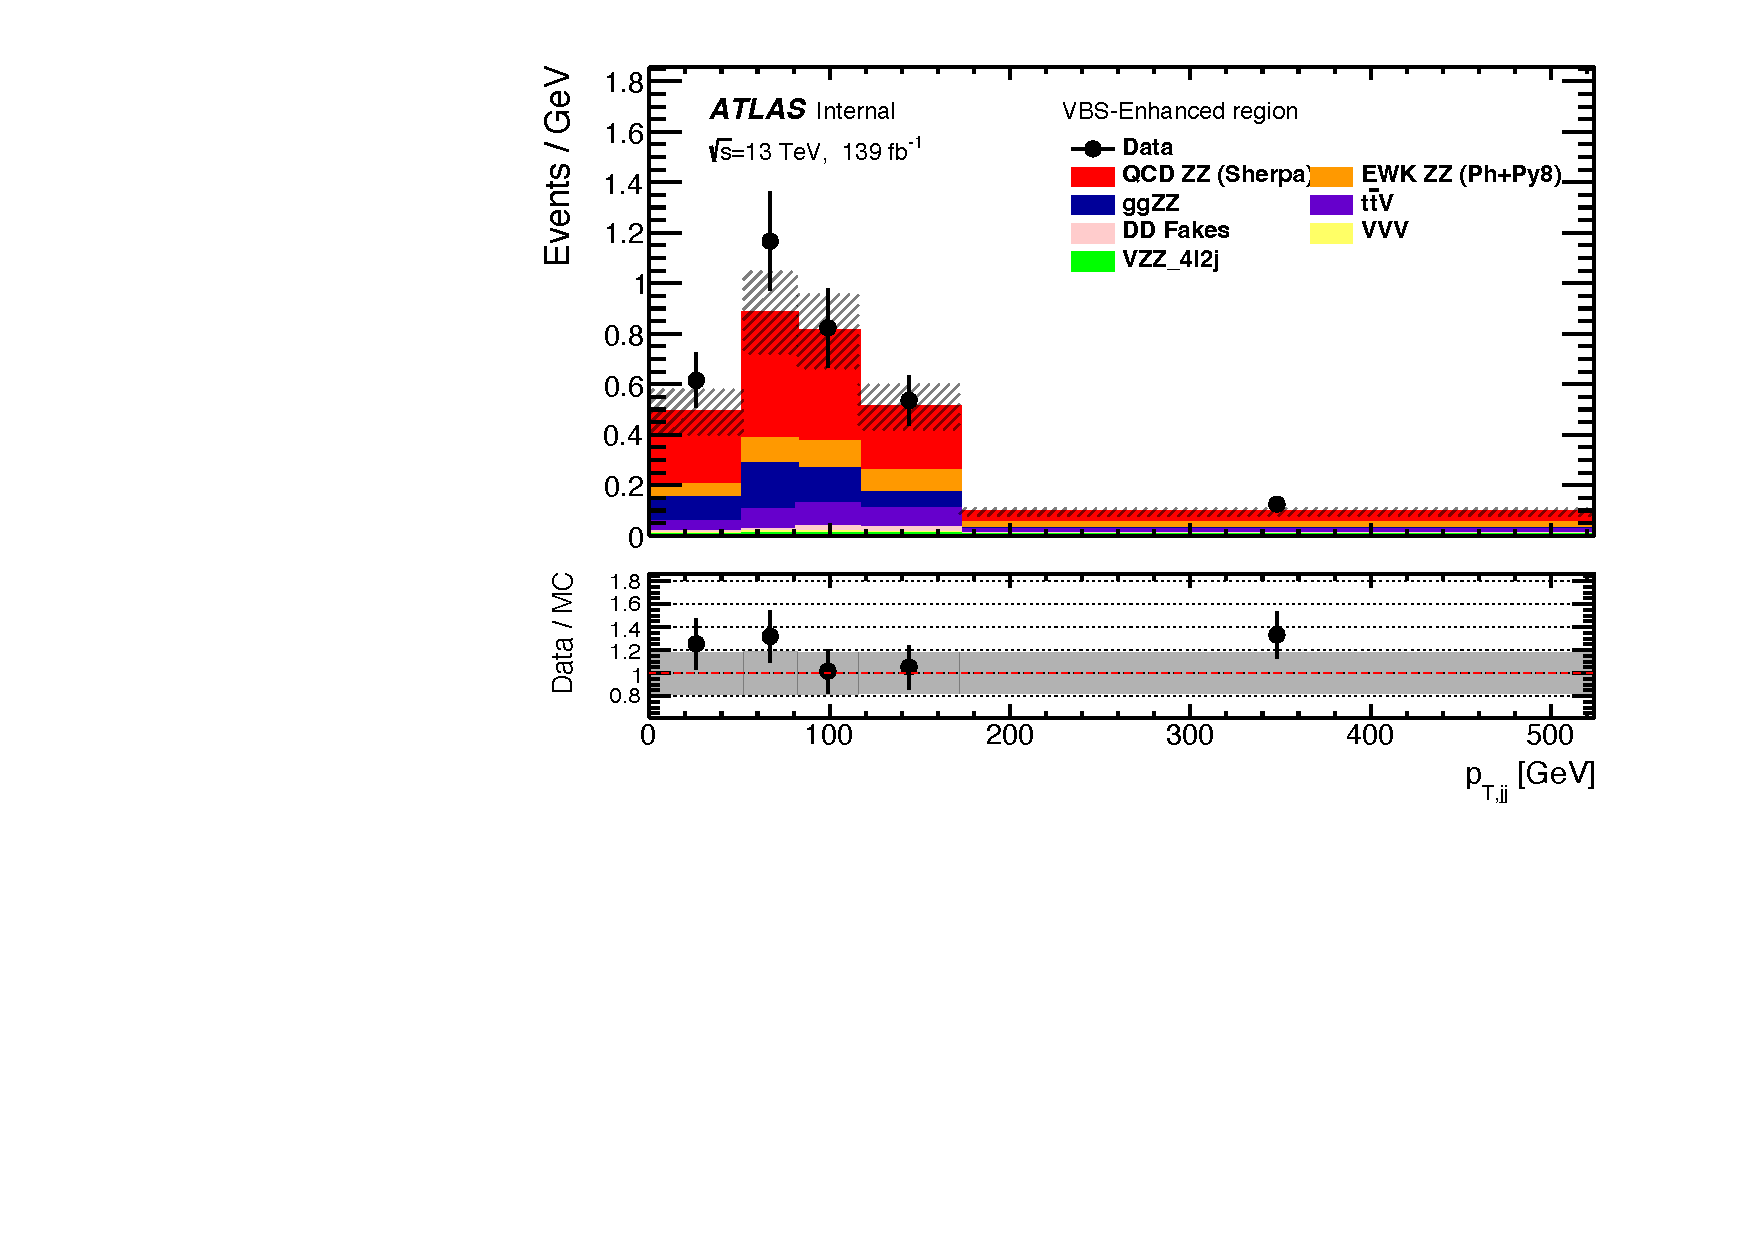
\includegraphics[width=.98\linewidth]{figures/Results/RecoDist_VBSEnhanced/reco_ptjj_SR.pdf}
        \caption{ \footnotesize{$p_{T,jj}$}: $\chi^2/NDF = 0.30$ }
    \end{subfigure}
    \begin{subfigure}{.49\textwidth}
        \centering
        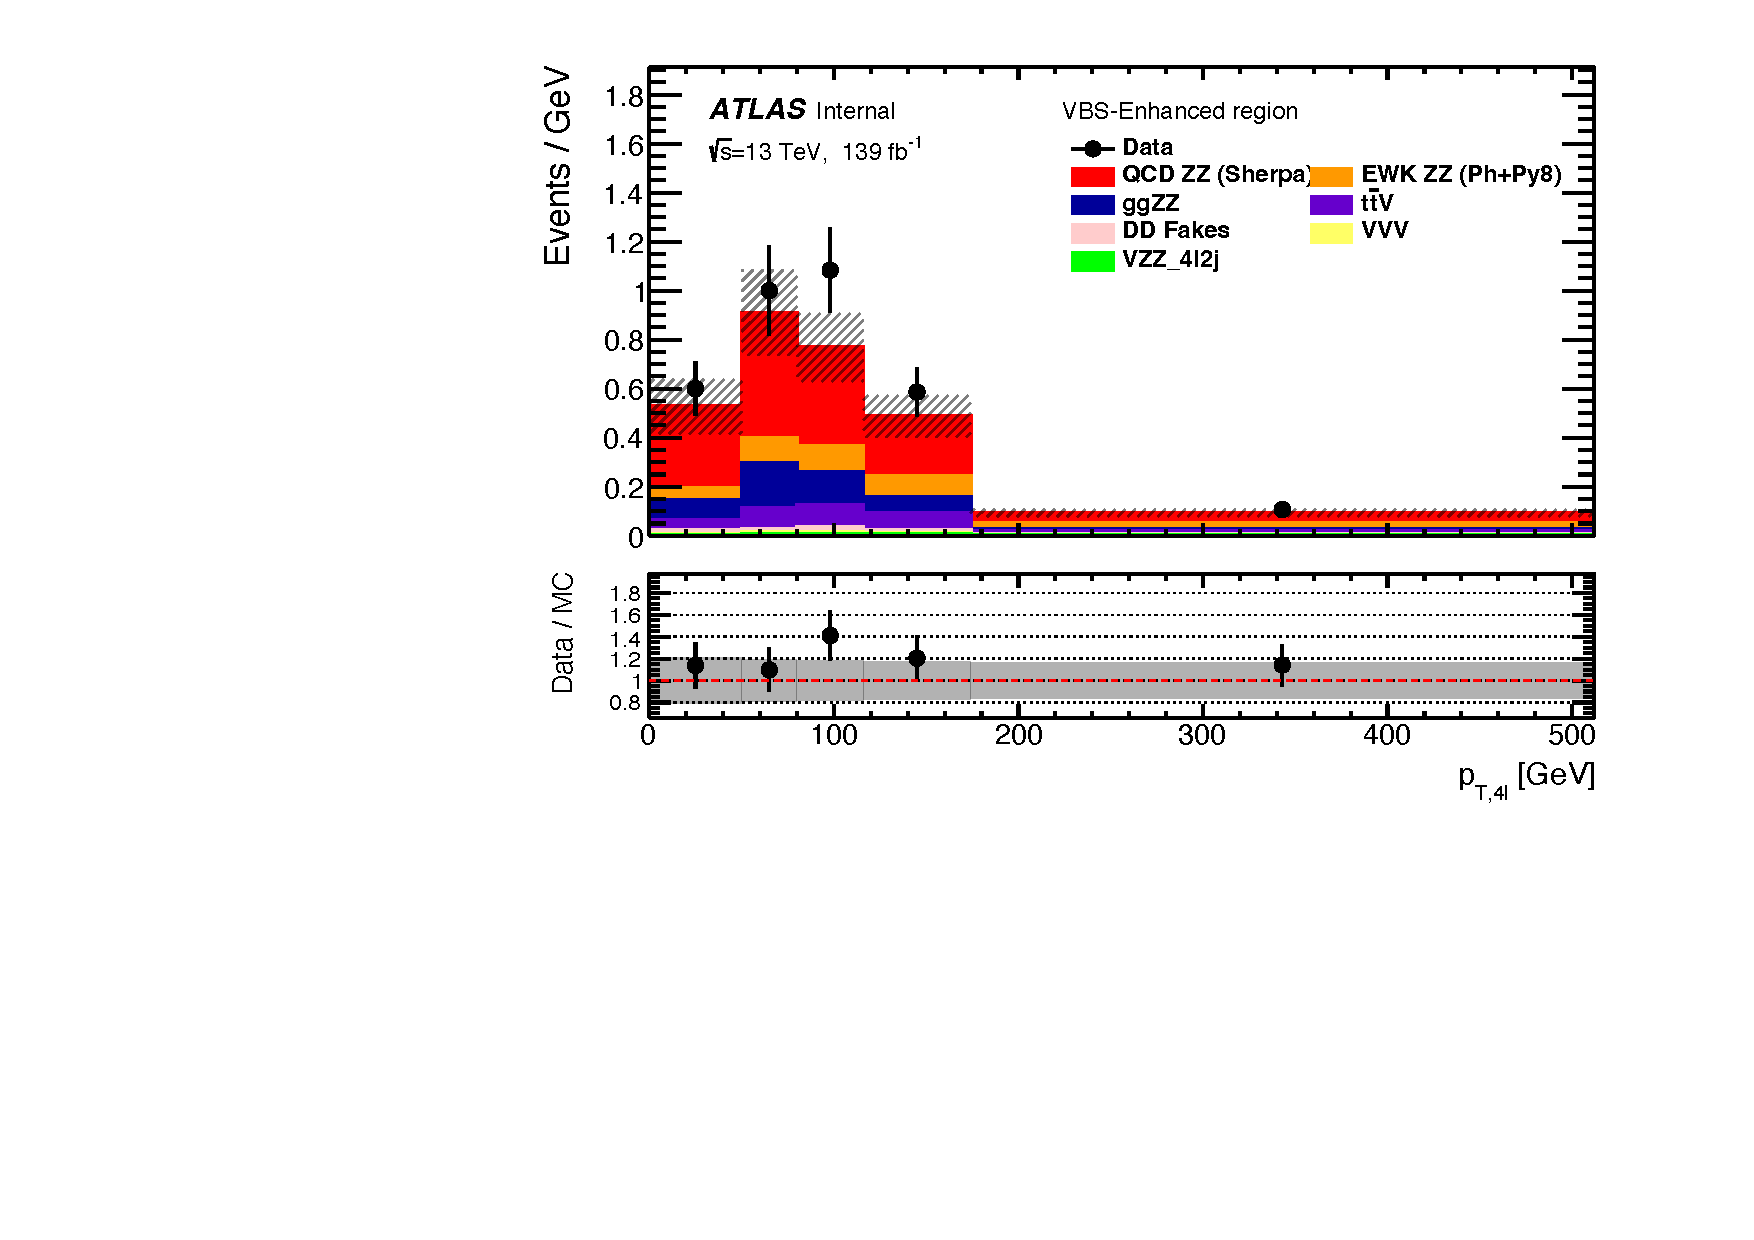
\includegraphics[width=.98\linewidth]{figures/Results/RecoDist_VBSEnhanced/reco_pt4l_SR.pdf}
        \caption{ \footnotesize{$p_{T,4\ell}$ }: $\chi^2/NDF = 0.15$ }
    \end{subfigure}\\
    \begin{subfigure}{.49\textwidth}
        \centering
        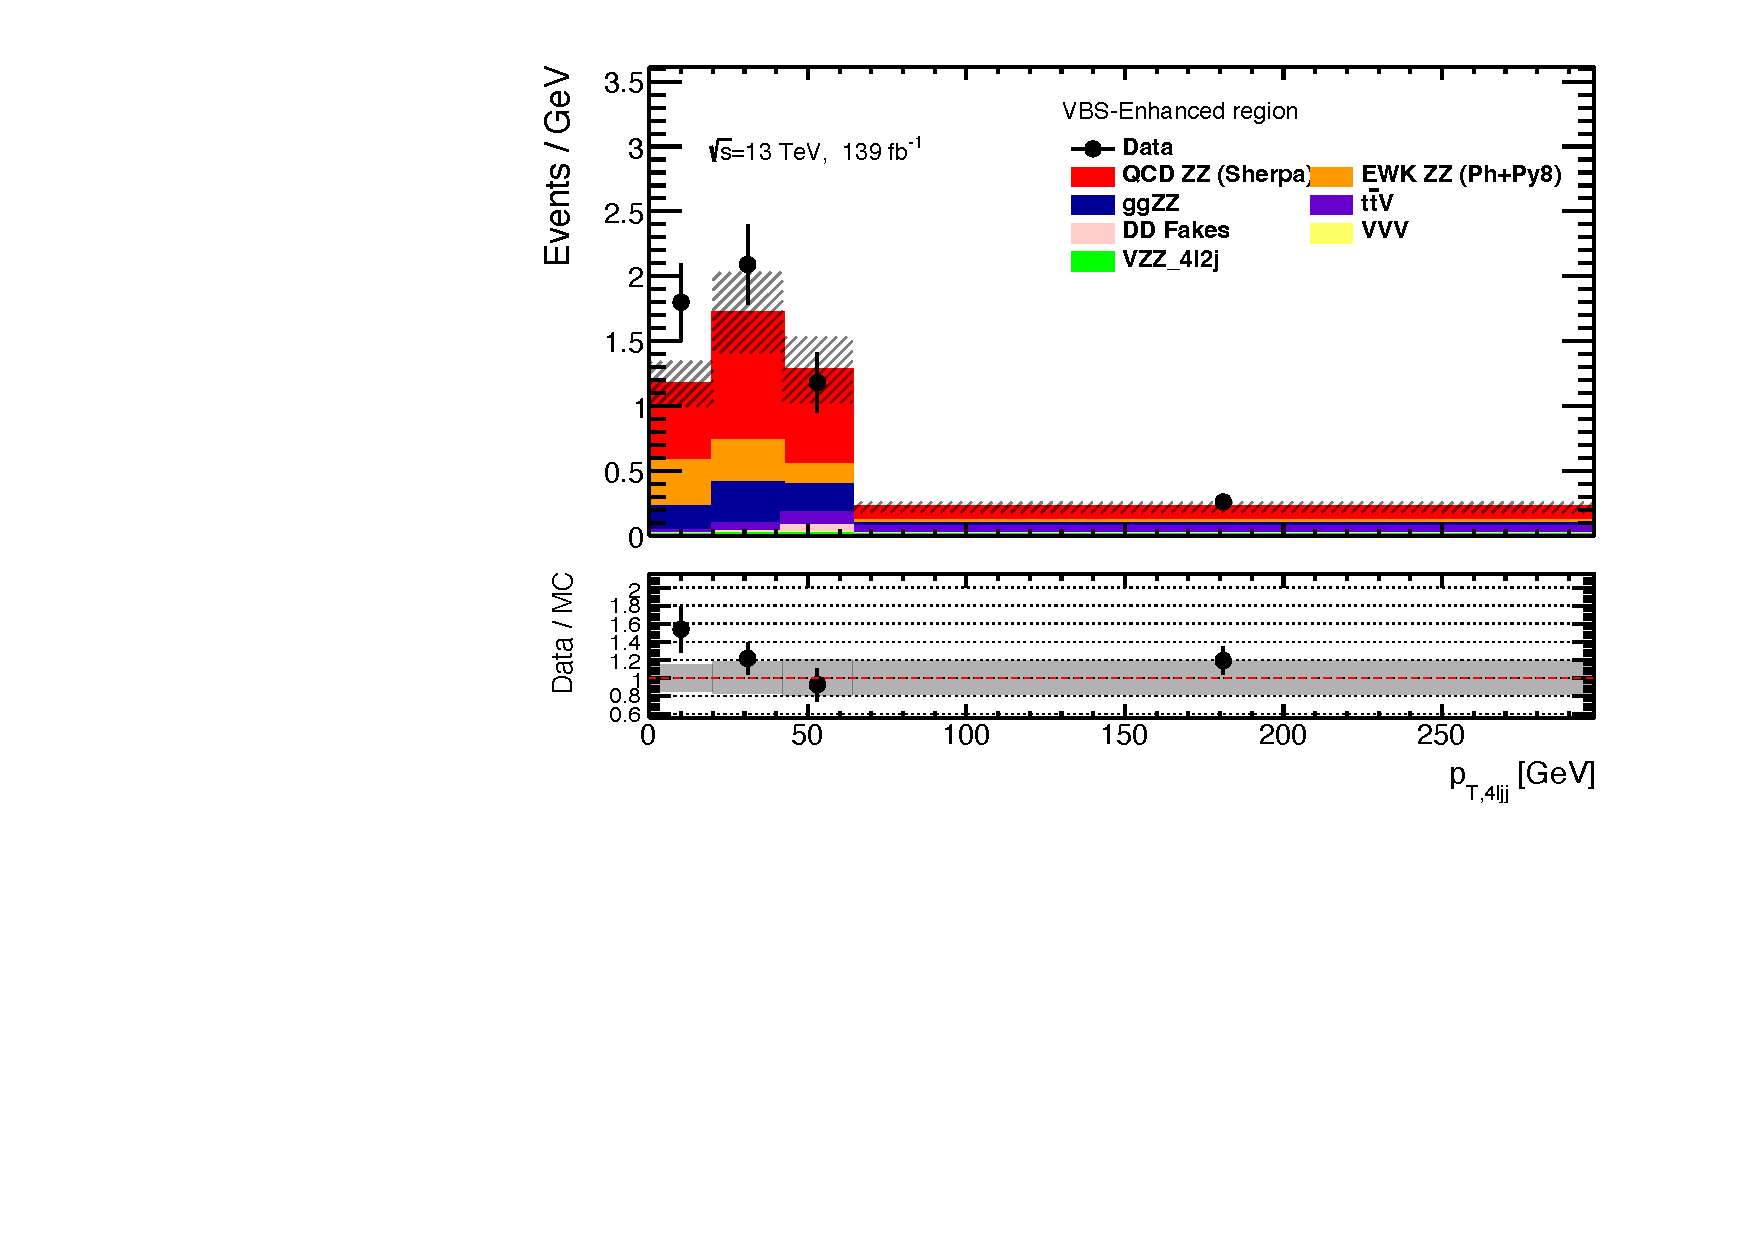
\includegraphics[width=.98\linewidth]{figures/Results/RecoDist_VBSEnhanced/reco_ptzzjj_SR.pdf}
        \caption{ \footnotesize{$p_{T,4\ell jj}$}: $\chi^2/NDF = 0.70$ }
    \end{subfigure}
    \begin{subfigure}{.49\textwidth}
        \centering
        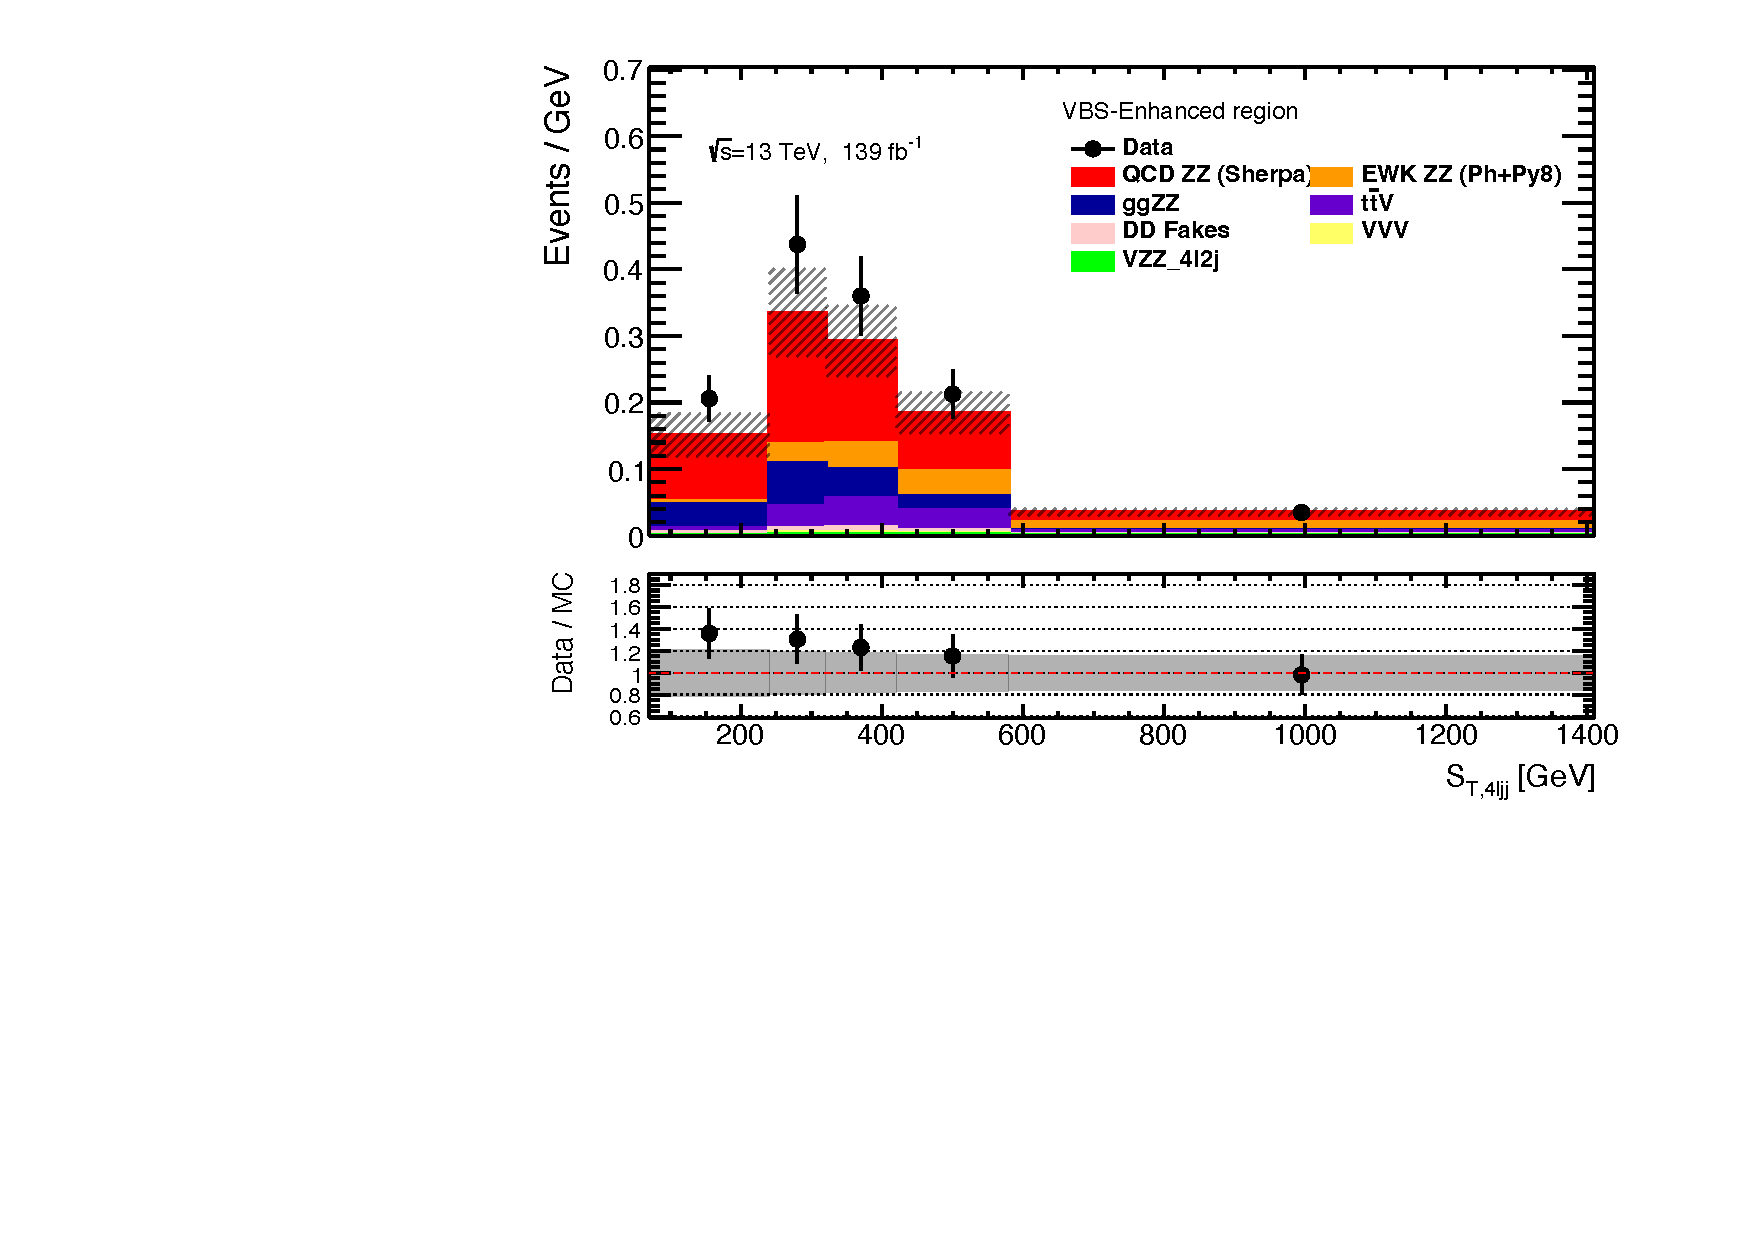
\includegraphics[width=.98\linewidth]{figures/Results/RecoDist_VBSEnhanced/reco_stzzjj_SR.pdf}
        \caption{ \footnotesize{$s_{T, 4\ell jj}$ }: $\chi^2/NDF = 0.24$ }
    \end{subfigure}
    \caption{Detector level distributions in the VBS-Enhanced region.}  \label{fig:reco_VBS_Enhanced_a}
\end{figure}

\begin{figure}[!htb]
    \centering
    \begin{subfigure}{.49\textwidth}
        \centering
        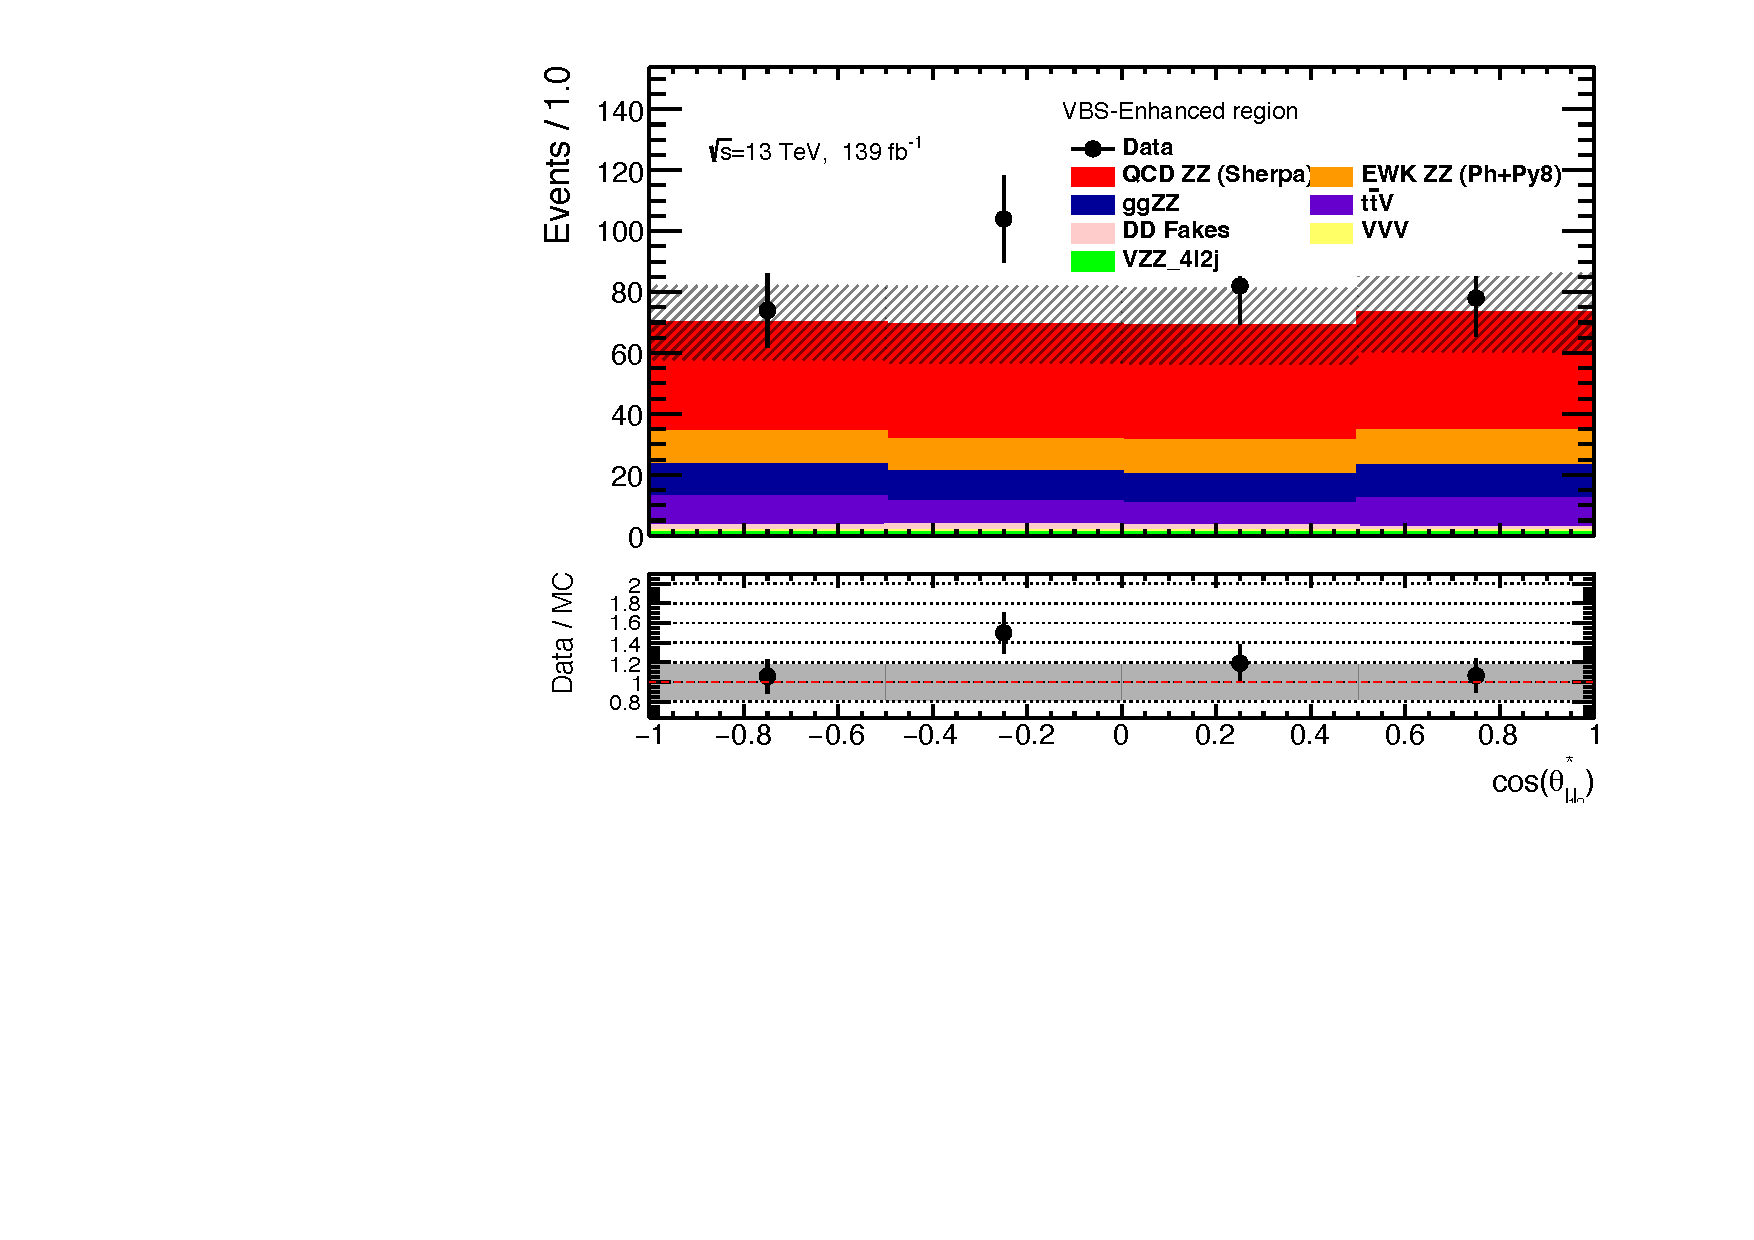
\includegraphics[width=.98\linewidth]{figures/Results/RecoDist_VBSEnhanced/reco_cosThetaStar1_SR.pdf}
        \caption{ \footnotesize{$\cos \theta^{*}_{\ell 1 \ell 2}$}: $\chi^2/NDF = 0.51$ }
    \end{subfigure}
    \begin{subfigure}{.49\textwidth}
        \centering
        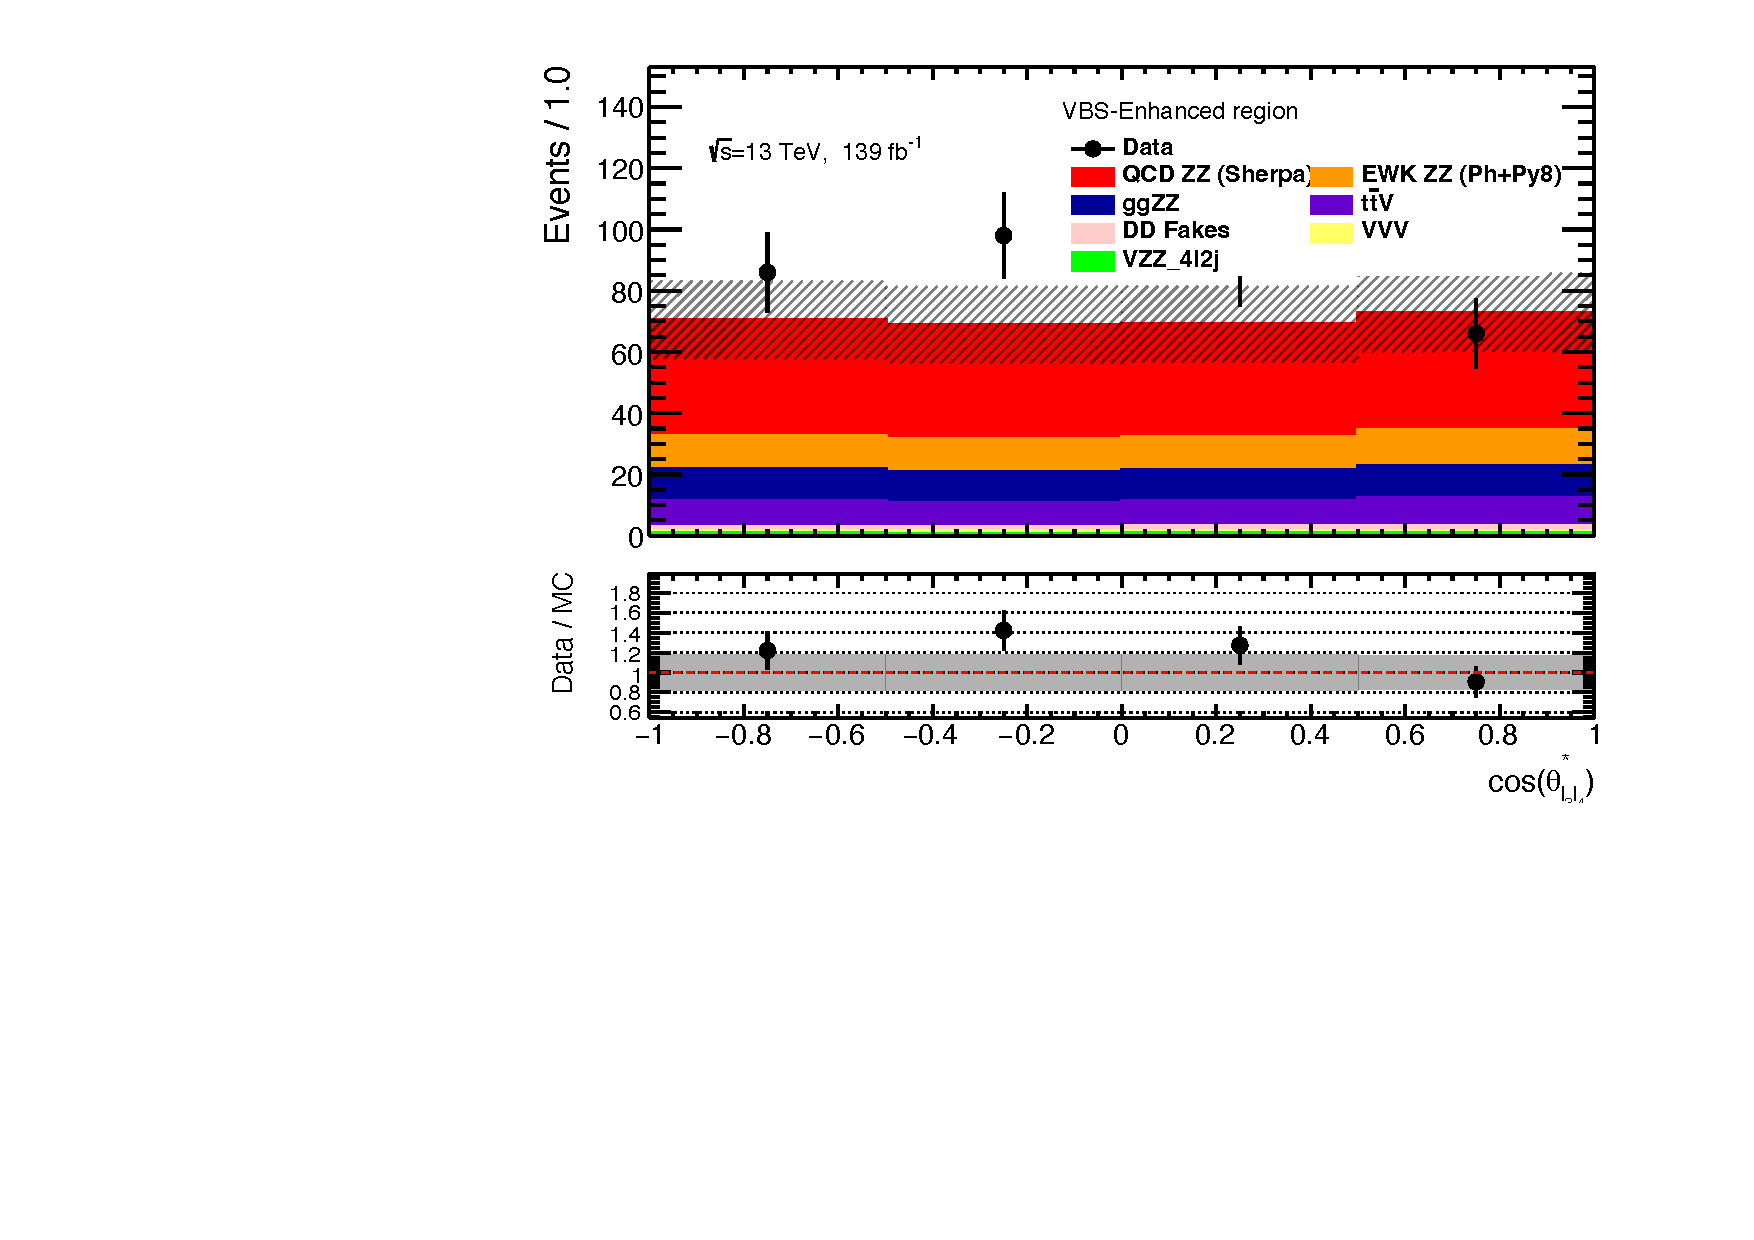
\includegraphics[width=.98\linewidth]{figures/Results/RecoDist_VBSEnhanced/reco_cosThetaStar3_SR.pdf}
        \caption{ \footnotesize{$\cos \theta^{*}_{\ell 3 \ell 4}$ }: $\chi^2/NDF = 0.61$ }
    \end{subfigure}\\
    \begin{subfigure}{.49\textwidth}
        \centering
        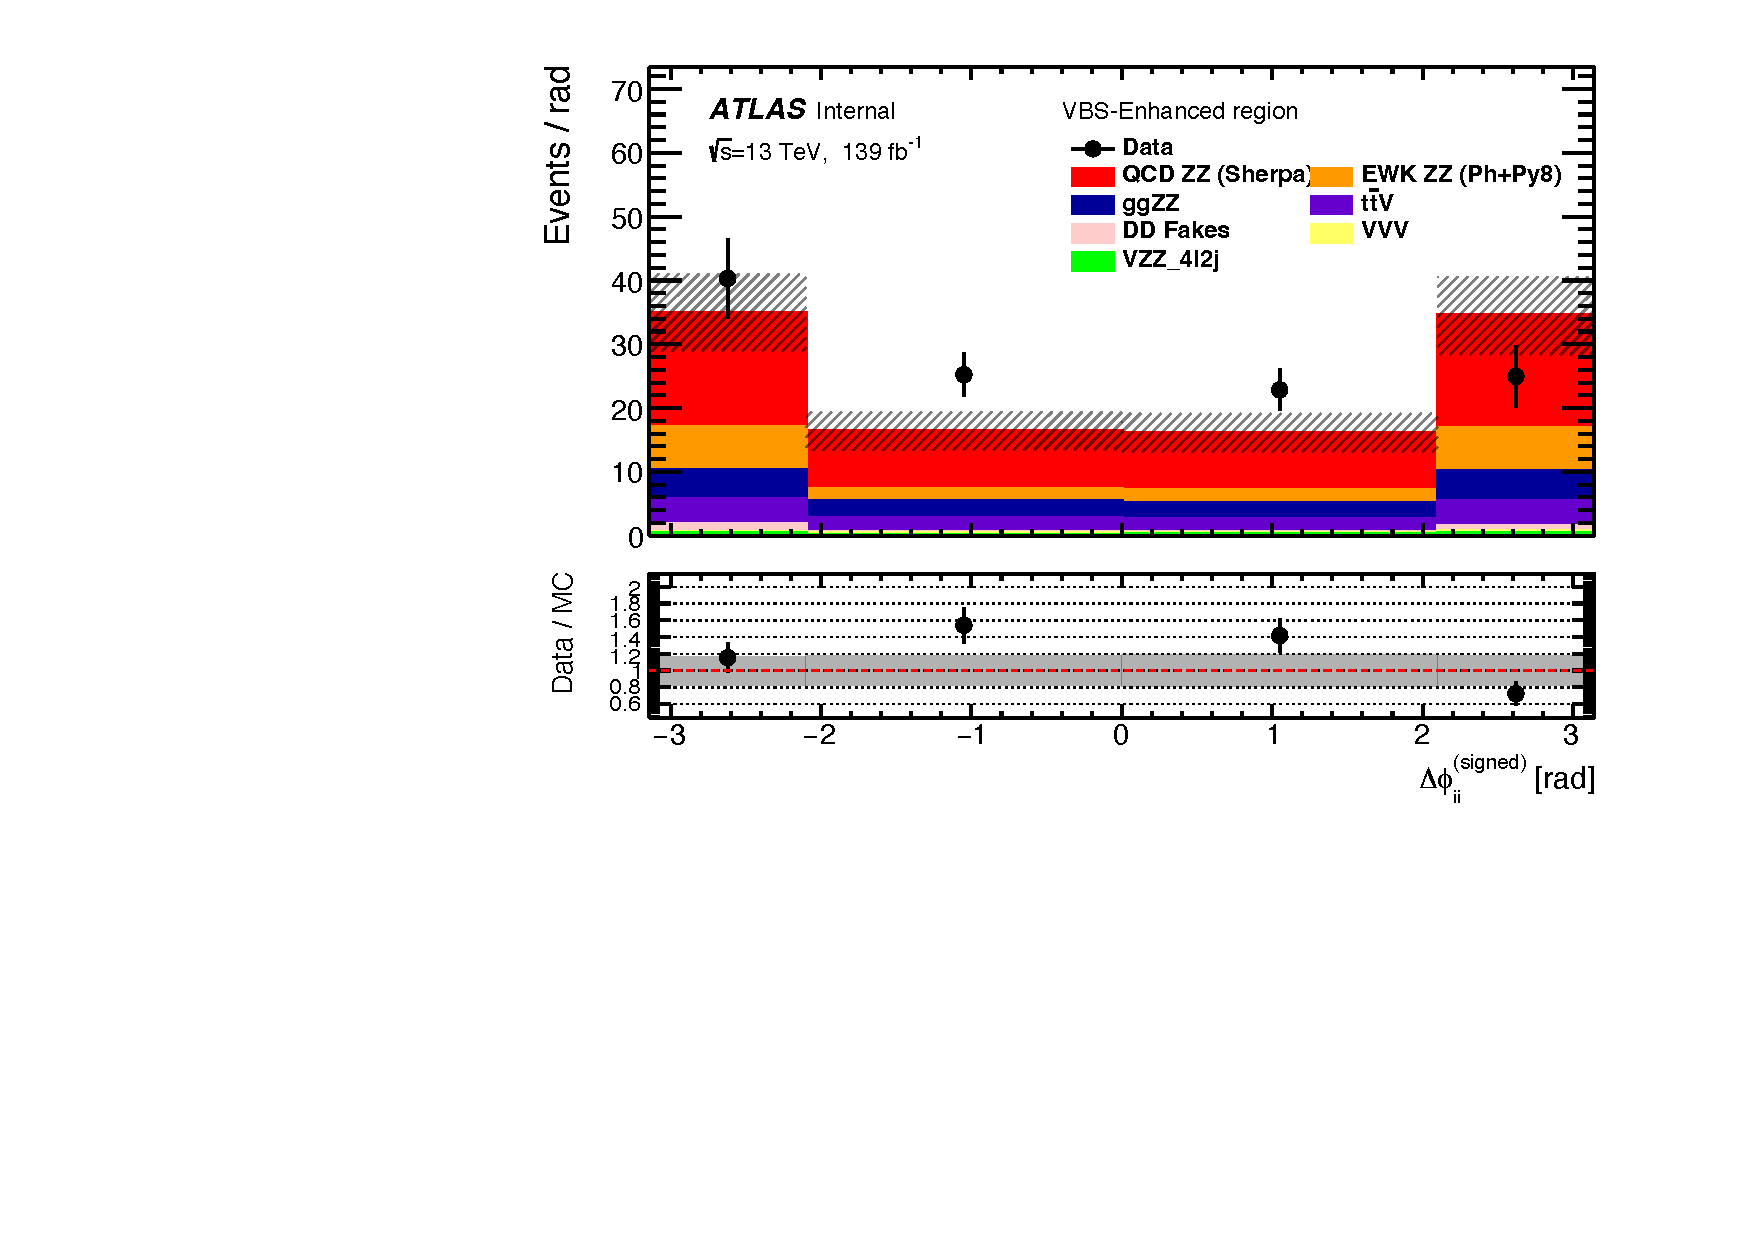
\includegraphics[width=.98\linewidth]{figures/Results/RecoDist_VBSEnhanced/reco_dphi_SR.pdf}
        \caption{ \footnotesize{$\Delta \phi _{jj}^{signed}$ }: $\chi^2/NDF = 1.69$ }
    \end{subfigure}
    \begin{subfigure}{.49\textwidth}
        \centering
        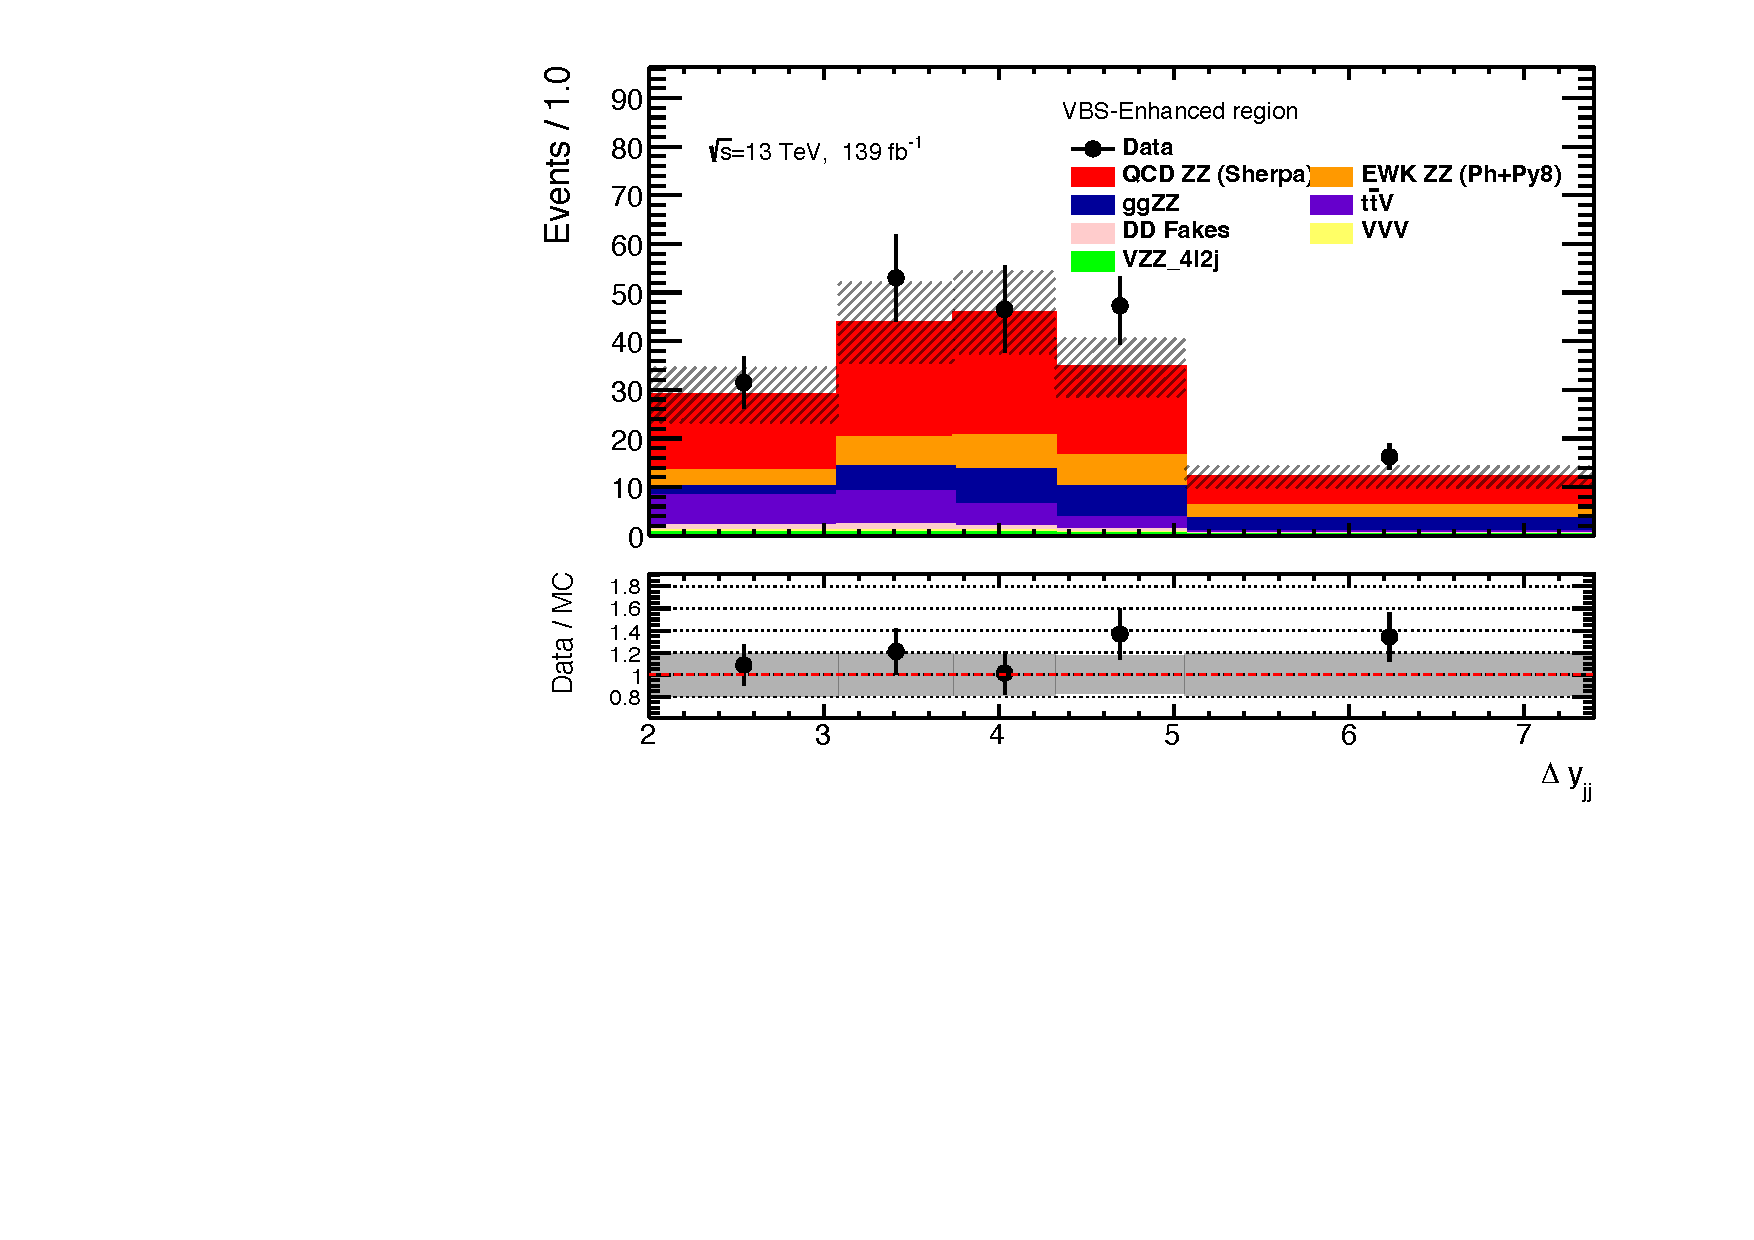
\includegraphics[width=.98\linewidth]{figures/Results/RecoDist_VBSEnhanced/reco_dy_SR.pdf}
        \caption{ \footnotesize{$\Delta y_{jj}$ }: $\chi^2/NDF = 0.26$ }
    \end{subfigure}\\
    \begin{subfigure}{.49\textwidth}
        \centering
        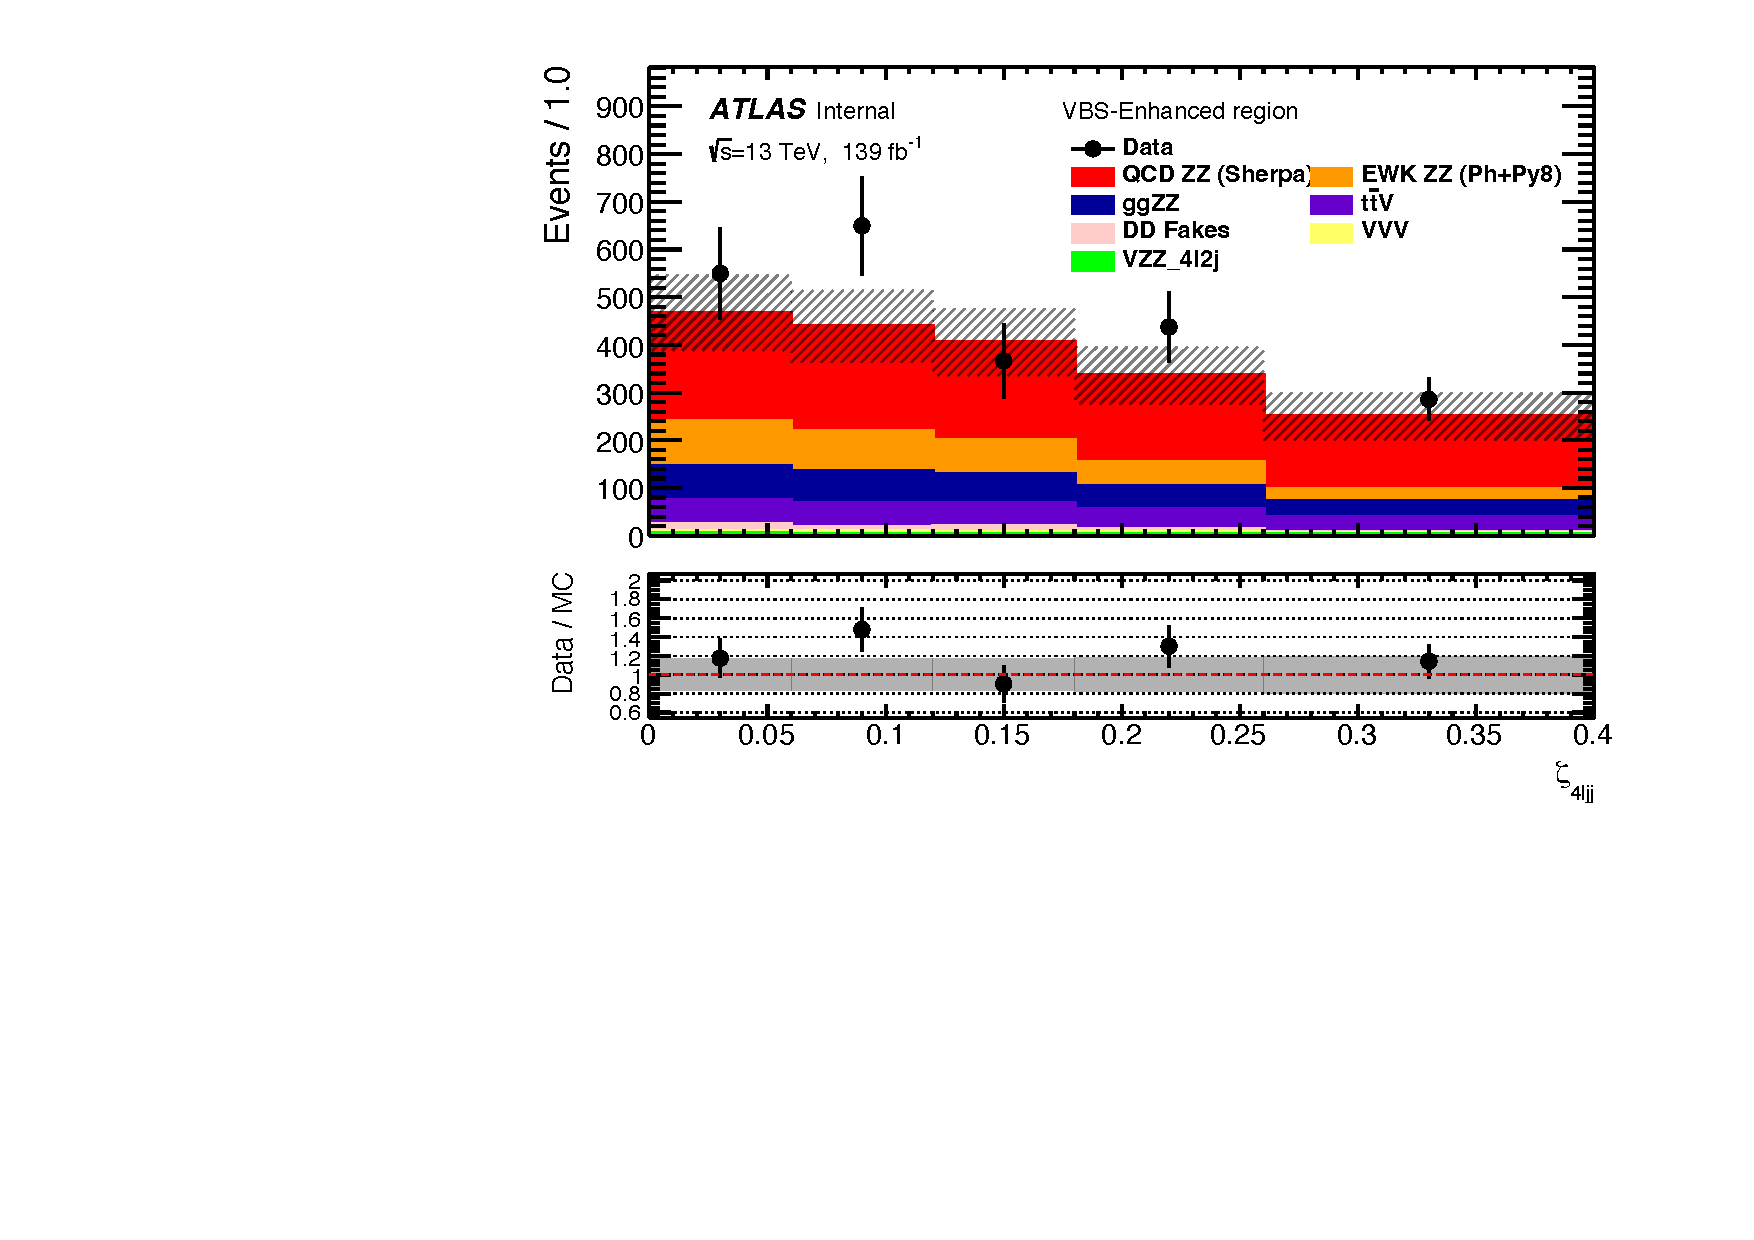
\includegraphics[width=.98\linewidth]{figures/Results/RecoDist_VBSEnhanced/reco_centrality_SR.pdf}
        \caption{ \footnotesize{$\zeta$ }: $\chi^2/NDF = 0.50$ }
    \end{subfigure}
    \caption{Detector level distributions in the VBS-Enhanced region.}  \label{fig:reco_VBS_Enhanced_b}
\end{figure}